% Apresentar as pontes que vc vai estudar. Apresenta só duas.

A fim de estudar os modelos e subsidiar as implementações, foram visitadas, na região sudeste do estado de Goiás — que abrange os municípios de Catalão, Ipameri, Nova Aurora, Domiciano Ribeiro, Goiandira, entre outros — algumas pontes de madeira, com o objetivo de caracterizar o estado atual dessas infraestruturas \ref{fig:pontes}. As dimensões das pontes selecionadas para este estudo são apresentadas na Tabela \ref{tab_pontes}.

\begin{figure}[htpb!]
    \centering
    \caption{Pontes inspecionadas.}
    \label{fig:pontes}

    \begin{subfigure}[t]{0.30\textwidth}
        \centering
        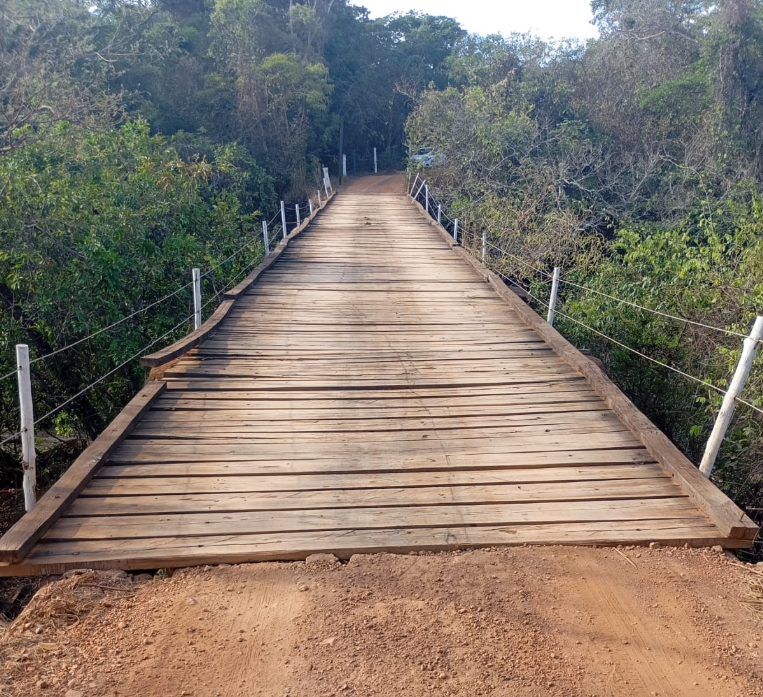
\includegraphics[width=\textwidth]{imgs/Rio do Braço.png}
        \caption{Ponte Rio do Braço}
        %\label{fig:ponte_a}
    \end{subfigure}
    %\hfill
    % \begin{subfigure}[t]{0.31\textwidth}
    %     \centering
    %     \includegraphics[width=\textwidth]{}
    %     \caption{Ponte R. Mascarenhas Morais}
    %     %\label{fig:ponte_b}
    % \end{subfigure}
    % \hfill
    \begin{subfigure}[t]{0.36\textwidth}
        \centering
        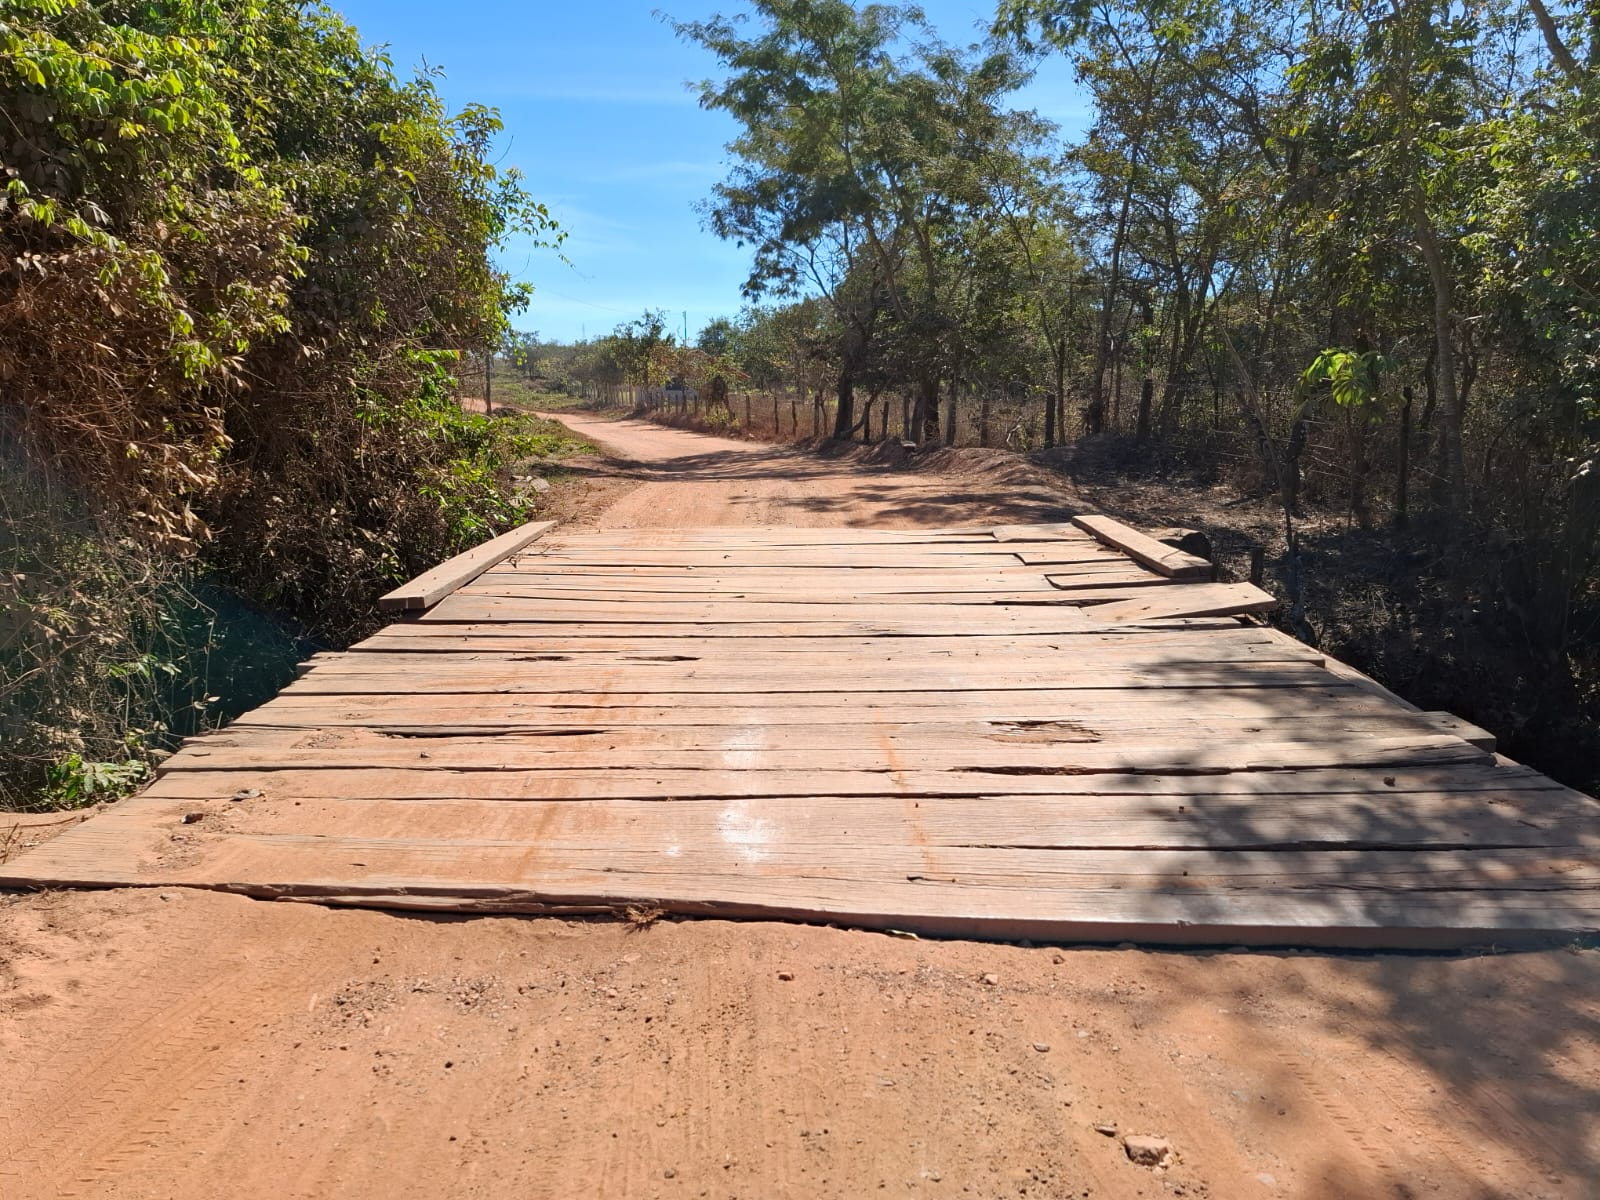
\includegraphics[width=\textwidth]{imgs/três bocas.jpg}
        \caption{Ponte Três Bocas}
        % \label{fig:ponte_c}
    \end{subfigure}
     % \legend{(a) Ponte Rio do Braço; (b) Ponte R. Mascarenhas Morais; (c) Ponte Três Bocas.}
\end{figure}

\begin{table}[htpb!]
\centering
\caption{Características das Pontes}
\label{tab_pontes}
\footnotesize
\begin{tabular}{
>{\centering\arraybackslash}m{1.8cm}
>{\centering\arraybackslash}m{1.5cm}
>{\centering\arraybackslash}m{1.5cm}
>{\centering\arraybackslash}m{2cm}
>{\centering\arraybackslash}m{1.5cm}
>{\centering\arraybackslash}m{2cm}
>{\centering\arraybackslash}m{2.5cm}
}
\hline
\textbf{Ponte} & \textbf{Comp.} & \textbf{Larg.} & \textbf{Madeira} & \textbf{Q. Long.} & \textbf{Dia. Long.} & \textbf{Pilares} \\ 
\hline
\multirow{2}{*}{Rio do Braço} & \multirow{2}{*}{42 m} & \multirow{2}{*}{3,50 m} & Eucalipto & \multirow{2}{*}{6} & \multirow{2}{*}{45--57} & \multirow{2}{*}{Pedra} \\
& & & Aroeira & & & \\ 
%\hline
\multirow{2}{*}{Três Bocas} & \multirow{2}{*}{6,40 m} & \multirow{2}{*}{3,50 m} & Aroeira & 3 & \multirow{2}{*}{43--54} & \multirow{2}{*}{Concreto} \\ 
& & & Angico & 6 & & \\
%\hline
% Ponte 03 & 7 m & 7 m & Aroeira & 6 & 44--53 & Pedra \\ 
\hline
\end{tabular}
\end{table}
   
    
Com base na configuração típica observada nessas estruturas, o sistema estrutural considerado consiste em um tabuleiro de madeira composto por pranchas longitudinais, apoiadas sobre vigas longitudinais circulares de madeira (longarinas), regularmente espaçadas. O tabuleiro está sujeito a ações permanentes (peso próprio) e ações variáveis associadas ao tráfego (carga móvel). As cargas atuantes no tabuleiro são transferidas para as longarinas de apoio e modeladas como carregamentos uniformemente distribuídos ao longo do vão. Uma representação esquemática do sistema estrutural é apresentada na Figura~\ref{fig:Ponte Frontal}.

\begin{figure}[h!]
    \centering
    \caption{Representação do sistema estrutural da ponte em madeira.}
    \label{fig:Ponte Frontal}
    \includegraphics[width=0.35\textwidth]{imgs/Ponte Frontal.png}\\   
    \vspace{0.2cm}
    \centering \small Fonte: Autoria própria, 2025.
\end{figure}








\subsection{Framework}
dsdspsmdsmpssdpsd46546466522

215551

\subsection{Dimensioanmento parámetrico}



% Para avaliação da confiabilidade e análise de custo foi adotado o problema de \textit{benchmark} descrito na Figura \ref{fig:toy1} que consiste em uma edificação hipotética em alvenaria estrutural composta por 7 paredes. A altura de cada pavimento é 2,80 m e também para efeito de cálculo fora considerado um carregamento de 10 pavimentos sobre as paredes do térreo apresentada na Figura \ref{fig:toy1}.

% \begin{figure}[htpb!]
% \centering
% 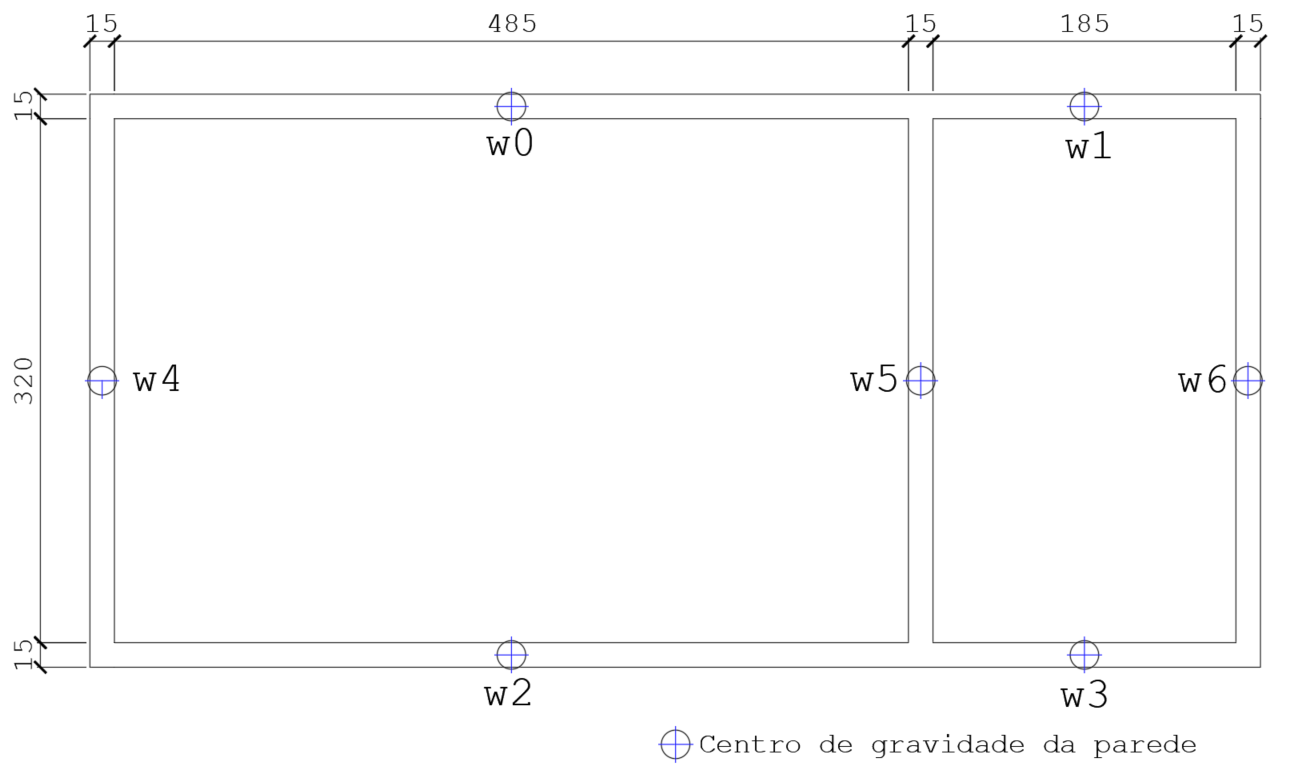
\includegraphics[width=0.9\textwidth]{imgs/benchmark1.png}
% \caption{Distribuição de paredes do edifício de alvenaria estrutural com dimensões em centímetros.}
% \label{fig:toy1}
% \end{figure}

% A Figura \ref{fig:toy2} apresenta os fatores de carregamento para o sistema intacto ($nlc$) e para a condição com remoção da parede $W_1$ ($r,w1$). No sistema sem remoção ($nlc$), o maior fator de carga é de 0,240, associado à parede $W_1$, indicando que esta é a mais solicitada na condição sem remoção de paredes. Já no sistema considerando a remoção da parede $W_1$ ($r,w1$), o maior fator de carga é de 0,285, referente à parede $W_5$. Esse aumento no fator de carregamento da parede $W_5$ decorre da redistribuição de esforços provocada pela remoção da parede $W_1$, resultando em um acréscimo na parcela de carga suportada pelas demais paredes.

% \begin{figure}[htpb!]
%     \centering
%     \begin{subfigure}[b]{0.48\textwidth}
%         \centering
%         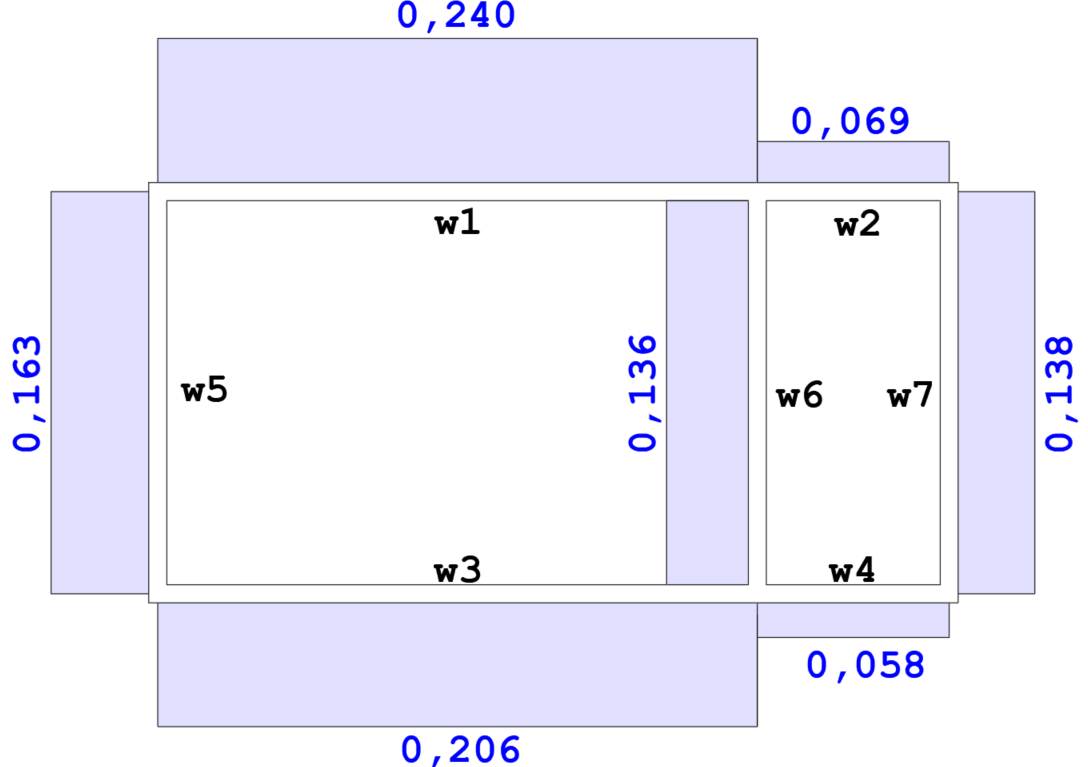
\includegraphics[width=\linewidth]{imgs/Sem remoção.png} % Substitua pelo seu arquivo
%         \caption{Sistema sem remoção de paredes}
%         \label{fig:toy2a}
%     \end{subfigure}
%     \hfill % Espaço entre as colunas
%     \begin{subfigure}[b]{0.48\textwidth}
%         \centering
%         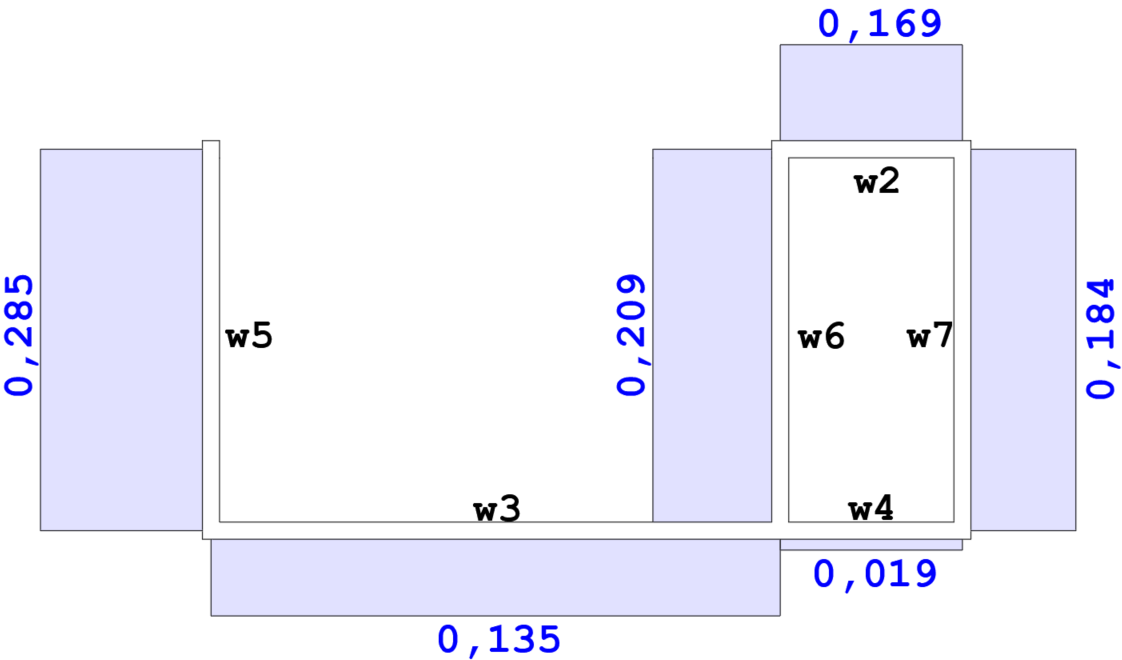
\includegraphics[width=\linewidth]{imgs/Com remoção.png} % Substitua pelo seu arquivo
%         \caption{Sistema com remoção da parede $W_1$}
%         \label{fig:toy2b}
%     \end{subfigure}
%     \caption{Fatores de esforço normal para sistema estrutural em paredes estruturais.}
%     \label{fig:toy2}
% \end{figure}

% Para a análise de confiabilidade do sistema estrutural foram adotadas as estatísticas apresentadas na Tabela \ref{tab:estatisticas}. No modelo considerado, $g$ representa o peso próprio da laje, enquanto $g_{ppl}$ corresponde à carga permanente adicional da laje, englobando revestimentos, argamassas e demais acabamentos fixos. O peso próprio das paredes é representado pela variável $g_{par}$.

% A carga variável de uso e ocupação da edificação para um período de referência de 50 anos é denotada por $q_k$, sendo adotado o valor de 1,50 kN/m², em conformidade com a ABNT NBR 6120. Para efeito de cálculo, foram considerados ainda os valores de 2,70 kN/m² para o peso próprio das paredes e 2,50 kN/m² para o peso próprio da laje. Já a carga $q_{apt}$ é a carga variável de uso e ocupação da edificação anual e será empregada na avaliação pós remoção da parede. A resistência característica do prisma de alvenaria ($f_{pk}$) representa o comportamento conjunto de blocos e argamassa. O fator de erro de resistência ($\theta_R$) expressa as incertezas relacionadas ao modelo de cálculo da resistência, enquanto o fator de erro de carregamento ($\theta_L$) representa as incertezas associadas à estimativa e modelagem das ações aplicadas.


% \begin{table}[htpb!]\footnotesize
% \centering
% \caption{Estatísticas das variáveis de projeto.}
% \label{tab:estatisticas}
% \begin{tabular}{c c c c c c}
% \toprule
% \textbf{Variável} & \textbf{Descrição} & \textbf{Média} & \textbf{CV} & \textbf{Distribuição} & \textbf{Referências} \\
% \midrule
% $g$ & Peso próprio da laje & $1,06 \cdot g$ & 0,12 & Normal & Santiago \textit{et al.} \cite{santiago_reliability-based_2020} \\
% $g_{ppl}$ & Carga permanente atuante nas lajes & $1,06 \cdot g_{ppl}$ & 0,12 & Normal & Santiago \textit{et al.} \cite{santiago_reliability-based_2020} \\
% $g_{par}$ & Carga permanente das paredes & $g_{par}$ & 0,02 & Normal & Isfeld \textit{et al.} \cite{isfeld_structural_2023} \\
% $q_{50}$ & Carga variável & $0,92 \cdot q_k$ & 0,25 & Gumbel máx. & Costa et al. \cite{costa_probabilistic_2022} \\
% $q_{apt}$ & Carga variável & $0,21 \cdot q_k$ & 0,76 & Gumbel máx. & Costa et al. \cite{costa_probabilistic_2022} \\
% $f_{pk}$ & Resistência característica do prisma & $1,36 \cdot f_{pk\text{}}$ & 0,24 & Normal & Santiago \textit{et al.} \cite{santiago_unreinforced_2024} \\
% $\theta_R$ & Erro de resistência & $0,95$ & 0,14 & Lognormal & Isfeld \textit{et al.} \ \cite{isfeld_structural_2023} \\
% $\theta_L$ & Erro de carga & $1$ & 0,05 & Lognormal & Costa et al. \cite{costa_probabilistic_2022} \\
% \bottomrule
% \end{tabular}
% \end{table}

% \subsection{Reinforced concrete versus Concrete Masonry: loss impact}

% A comparação entre estruturas de concreto armado e de alvenaria estrutural em cenários de perda de elementos revela diferenças marcantes no modo como os esforços se redistribuem. Na alvenaria estrutural, as cargas são predominantemente transmitidas por compressão axial e distribuídas ao longo das paredes. Essa configuração proporciona uma redistribuição mais homogênea, na qual a perda localizada de uma parede resulta em acréscimos de esforço relativamente modestos nos elementos adjacentes, como evidenciado na figura \ref{fig:toy2} desse artigo.

% Em contraste, nas estruturas de concreto armado compostas por vigas e pilares, a hiperestaticidade implica em redistribuições mais intensas. A retirada de um pilar ou apoio transfere esforços significativos para elementos vizinhos, gerando discrepâncias consideráveis em termos de flexão e esforço cortante. Embora a ductilidade do concreto armado e a formação de rótulas plásticas permitam ao sistema resistir temporariamente, o preço a pagar é a concentração elevada de esforços em pontos críticos, o que pode comprometer a durabilidade e acelerar o processo de degradação.

% \begin{figure}[htpb!]
% \centering
% 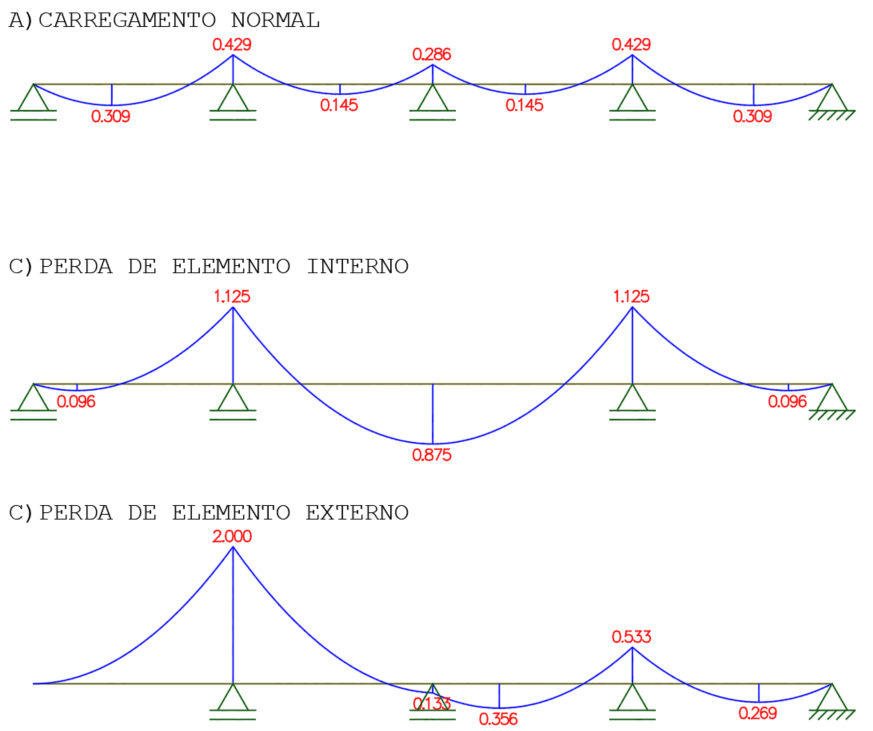
\includegraphics[width=0.8\textwidth]{imgs/intact_bean.png}
% \caption{Momentos fletores em viga contínua de quatro vãos: (a) Viga contínua intacta, todos os apoios presentes; (b) Redistribuição de esforços após remoção de um apoio central; (c) Redistribuição de esforços após remoção de um apoio lateral.}
% \label{fig:toy5}
% \end{figure}

% Os resultados obtidos em análises simplificadas no Ftool, com aplicação de carga unitária de 1 kN/m, ilustram esse contraste (figura \ref{fig:toy5}), enquanto nas paredes de alvenaria a variação de esforços normais se mantém em níveis relativamente uniformes após a perda de um elemento, em vigas e pilares de concreto armado surgem picos localizados de solicitação. Portanto, apesar da menor ductilidade, a alvenaria estrutural apresenta redistribuição mais equilibrada e previsível, minimizando as discrepâncias de esforços e reduzindo a vulnerabilidade a concentrações críticas em comparação às estruturas de concreto armado.

% \subsection{O projeto da edificação e avaliação da confiabilidade}

% A estrutura foi inicialmente projetada considerando a equações \eqref{eq:g_normal} e \eqref{eq:g_excepcional}. A Tabela \ref{tab:proj_alv1} apresenta os resultados para o valor de resistência de prisma necessária $\left(f_{pk}\right)$ para os carregamentos característicos indicados. Para a situação normal de carregamento e sem remoção de parede ($nlc$) foi avaliado o índice de confiabilidade da estrutura $\left(\beta_{nlc}\right)$. Após a remoção da parede estrutural $W1$ ($r,w1$) o índice de confiabilidade da estrutura $\left(\beta_{r,w1}\right)$ foi reavaliado. Na Tabela \ref{tab:proj_alv1} $g_{ppl}$ é calculado usando a equação \eqref{eq:gppl}.

% \begin{equation}
% g_{} = \frac{q_k}{L/D}
% \label{eq:gppl}
% \end{equation}

% \begin{table}[htpb!]
% \centering
% \caption{Resistências de prisma e índice de confiabilidade para o projeto estrutural em alvenaria considerando a equação \eqref{eq:g_normal}.}
% \label{tab:proj_alv1}
% \begin{tabular}{c c c c c c c}
% \toprule
% \textbf{L/D} & $g_{ppl} (MPa) $& $f_{bk}$ (MPa) & $f_{pk}$ (MPa)& $\beta_{nlc}$ & $\beta_{r,w1}$ & $\downarrow \Delta$ (\%)\\
% \midrule
% 1,00 & 1,50 & 6,00 & 4,50 & 2,59 & 1,99 & 23,4 \\
% 0,80 & 1,88 & 6,00 & 4,50 & 2,56 & 1,93 & 24,5 \\
% 0,60 & 2,50 & 6,00 & 4,50 & 2,51 & 1,85 & 26,5 \\
% 0,50 & 3,00 & 6,00 & 4,50 & 2,47 & 1,78 & 28,2 \\
% \bottomrule
% \end{tabular}
% \end{table}

% Observa-se que o índice de confiabilidade apresenta redução progressiva à medida que a carga permanente é elevada. Nos testes apresentados, essa redução foi, em média, da ordem de 25,65\%. Tal comportamento evidencia que o dimensionamento realizado conforme o método prescrito pela ASCE 7 \cite{american_society_of_civil_engineers_asce_asce_2013} pode conduzir a configurações estruturais associadas a probabilidades de falha relativamente elevadas, uma vez que valores de $\beta$ inferiores a 2,0 já se aproximam do limite de confiabilidade alvo geralmente aceito para elementos em regime de serviço. Nesse sentido, pode-se afirmar que os coeficientes parciais de segurança conservadores e o elevado grau de redundância característico das edificações em alvenaria estrutural tendem a mascarar os efeitos deletérios decorrentes da redistribuição de esforços após a remoção discricionária de uma ou mais paredes. Apesar disso é válido salientar que eventos de remoção discricionária de uma segunda parede são eventos com baixa probabilidade de ocorrência.

% \subsection{Análise de risco}

% Para analisar os efeitos da otimização de risco quando comparado ao método proposto pela ASCE 7 \cite{american_society_of_civil_engineers_asce_asce_2013} considera-se a proposta de Beck et al. \cite{beck_confiabilidade_2019} e Beck et al. \cite{beck_risk-based_2020} para construção da função objetivo conforme equação \eqref{eq:otm_risco}.

% \begin{equation}
% C_{ET}(\mathbf{\lambda_{pc}}) = C_C(\mathbf{\lambda_{pc}}) + C_{nlc} \cdot p_{c,nlc}(\mathbf{\lambda_{pc}}) + C_{ld} \cdot p_{c,ld}(\mathbf{\lambda_{pc}})
% \label{eq:otm_risco}
% \end{equation}

% Onde $C_{ET}$ é o custo total da edificação, $C_C$ o custo de construção da edificação. $C_{nlc}$ é o custo da falha total do sistema sob condições normais de carregamento. $C_{ld}$ é o custo da falha total do sistema dado um dano local prévio. $p_{c,nlc}$ e $p_{c,ld}$ são as probabilidades associadas aos eventos de colapso total da estrutura para condições normais de carregamento e um dano local, respectivamente. 

% As equações \eqref{eq:otm_risco_cc} a \eqref{eq:otm_risco_cld} representam os custos de construção e de falha. No caso os custos de falha são proporcionais ao custo de construção $C_C$.

% \begin{equation}
% C_C(\mathbf{\lambda_{pc}}) = \lambda_{pc}
% \label{eq:otm_risco_cc}
% \end{equation}

% \begin{equation}
% C_{nlc}(\mathbf{\lambda_{pc}}) = k \cdot \lambda_{pc}
% \label{eq:otm_risco_cnlc}
% \end{equation}

% \begin{equation}
% C_{ld}(\mathbf{\lambda_{pc}}) = k \cdot \lambda_{pc}
% \label{eq:otm_risco_cld}
% \end{equation}

% As equações \eqref{eq:otm_risco_pcnlc} e \eqref{eq:otm_risco_pcld} representam as probabilidades associadas aos eventos de falha on índices "NLC" corresponde a situação de condições normais de carregamento e "LD" a condição de dano local. Para este exemplo o dano local assumido consiste na remoção da parede $W_1$. 

% \begin{equation}
% p_{c,nlc}(\mathbf{\lambda_{PC}}) = P\left(C|NLC\right) \cdot P\left(NLC\right) 
% \label{eq:otm_risco_pcnlc}
% \end{equation}

% \begin{equation}
% p_{c,ld}(\mathbf{\lambda_{PC}}) = P\left(C|LD\right) \cdot P\left(LD\right) 
% \label{eq:otm_risco_pcld}
% \end{equation}

% Será considerado que a probabilidade de ocorrência do evento condições normais de carregamento ("NLC") é unitária e que a probabilidade de ocorrência de uma dano local varia entre $p_{ld}^{\min} \leq p_{ld} \leq 1$ onde $p_{ld}^{\min}$ é $5 \times 10^{-6}$ conforme Beck et al. \cite{beck_risk-based_2020}. As probabilidades $P\left(C|NLC\right)$ e $P\left(C|LD\right)$ são determinadas usando índice de Cornell conforme descrito na seção \ref{sec:confia}.

% Portanto o problema de otimização em minimizar o custo total da edificação em função de um custo de referência $\lambda_{pc}$, conforme equação \eqref{eq:otm_risco_min}. 

% \begin{equation}
% \begin{aligned}
% \text{Determinar } \lambda_{pc}^*, \\
% \text{minimizando} C_{TE}(\lambda_{pc}), \\
% \text{sujeito a: } \lambda_{pc} > 0.
% \end{aligned}
% \label{eq:otm_risco_min}
% \end{equation}


% \subsection{Arquitetura}
% O software é desenvolvido na linguagem Python, adotando uma arquitetura cliente-servidor. No lado do cliente, é disponibilizada uma interface web para entrada e visualização de dados, construída com a biblioteca Streamlit, o que resulta em uma interface simples, direta e intuitiva para o usuário. Já no lado do servidor, concentra-se todo o processamento computacional, englobando os cálculos estruturais determinísticos, como a verificação de tensões normais, flechas e esforços cortantes em elementos de madeira, bem como a análise probabilística, realizada por meio da implementação do método FORM (\textit{First-Order Reliability Method}) para a avaliação da confiabilidade estrutural.
% A escolha da linguagem Python deve-se, principalmente, ao seu amplo ecossistema de bibliotecas voltadas para análises numéricas e probabilísticas, além de sua ampla aceitação e utilização no meio acadêmico e científico, o que favorece a reprodutibilidade, a manutenção e a evolução do sistema.
% O fluxo de avaliação do gêmeo digital é organizado em três categorias principais de atividades: (a) o carregamento do cenário de análise desejado, no qual são definidos os dados geométricos, mecânicos e de carregamento da estrutura; (b) a escolha do nível de risco adotado, que estabelece os critérios de confiabilidade e segurança a serem considerados na avaliação; e (c) a aplicação do conceito de evidência e sua propagação em uma rede complexa, permitindo a integração das informações determinísticas e probabilísticas no processo de tomada de decisão. Cada uma dessas etapas é detalhada de forma a fornecer uma visão geral do funcionamento do gêmeo digital aplicado à análise do planejamento estrutural proposto.



% \subsection{Cenários de Upload de Conjunto de Dados e Método do Caminho Crítico}
% No contexto de cenários de upload de conjuntos de dados, o código foi estruturado para operar a partir de vetores de amostras que representam diferentes realizações possíveis das variáveis aleatórias do problema. Essas amostras podem ser interpretadas como cenários importados de um conjunto de dados externo, como planilhas ou bases de dados previamente preparadas. Cada linha do array \texttt{samples} corresponde a um cenário independente, contendo valores associados às cargas permanentes, cargas variáveis, resistências mecânicas e módulo de elasticidade. Esse formato é compatível com arquiteturas em que os dados são inicialmente organizados, validados e, posteriormente, carregados para processamento, de forma análoga ao upload de arquivos em aplicações interativas. A função \texttt{obj\_confia} concentra essa etapa, pois recebe todas as amostras simultaneamente e avalia, cenário a cenário, a função estado limite, retornando um vetor \texttt{g} que expressa a margem de segurança estrutural associada a cada realização.

% A consistência dos dados é garantida implicitamente pela própria estrutura do modelo. Assim como ocorre em sistemas de upload de cenários, nos quais colunas duplicadas, ausentes ou mal definidas inviabilizam a análise, cada posição do vetor de amostras possui um significado físico específico. Caso a ordem ou a quantidade de variáveis não seja respeitada, o modelo deixa de representar adequadamente o comportamento estrutural da viga. Dessa forma, a correta definição do \textit{dataset} é fundamental para que o método de confiabilidade forneça resultados fisicamente coerentes, como índices de confiabilidade $\beta$ e probabilidades de falha realistas.

% A parte determinística do código constitui a base da avaliação de cada cenário. Funções como \texttt{prop\_madeiras}, \texttt{momento\_max\_carga\_permanente}, \texttt{momento\_max\_carga\_variavel} e \\\texttt{coef\_impacto\_vertical} são responsáveis pelo cálculo das propriedades geométricas da seção e dos esforços internos a partir dos dados de entrada. Na sequência, são realizadas as verificações normativas de flexão, flecha e cisalhamento. Esse encadeamento de cálculos pode ser associado ao conceito de caminho crítico, no sentido de que existe uma sequência lógica obrigatória de etapas que deve ser respeitada para que a verificação estrutural seja válida. Caso alguma dessas etapas seja mal definida ou apresente inconsistências, todas as verificações subsequentes perdem seu significado físico.

% Dentro dessa lógica, a função \texttt{checagem\_longarina\_madeira\_flexao} pode ser interpretada como o caminho crítico do modelo estrutural. Ela reúne o cálculo dos esforços solicitantes, as combinações de ações, a aplicação do coeficiente de impacto vertical e, por fim, as verificações de estado limite. De forma análoga ao Método do Caminho Crítico no planejamento de projetos, em que o prazo total é governado pelas atividades críticas, a segurança global da longarina é governada pela condição mais desfavorável entre as verificações. O valor da função estado limite $g$ traduz exatamente esse ponto crítico, pois representa a diferença entre a resistência disponível e a solicitação atuante.

% Quando a análise probabilística é acionada, por meio da função \texttt{confia\_flexao\_pura}, o código passa a considerar explicitamente as incertezas associadas às variáveis de entrada. Para isso, são adotadas distribuições estatísticas, assumindo-se distribuições normais com coeficiente de variação de 10\%. O método FORM é então empregado para identificar o ponto mais provável de falha, que pode ser interpretado como o cenário crítico no espaço probabilístico. De maneira análoga ao conceito de caminho crítico em cronogramas, esse ponto domina o comportamento global do sistema, uma vez que pequenas variações em sua vizinhança provocam alterações significativas na probabilidade de falha.

% No que se refere à arquitetura da ferramenta, o \textit{dataset} da viga foi concebido para permitir três tipos distintos de dimensionamento: à flexão, à flecha e ao cisalhamento. Cada um desses modos de dimensionamento segue o mesmo fluxo lógico de avaliação determinística e, posteriormente, de análise de confiabilidade. A partir dessa estrutura, a ferramenta incorpora seis funcionalidades principais, combinando o dimensionamento da seção e a análise de confiabilidade para os três tipos de verificação. Essa abordagem integrada permite não apenas verificar se a viga atende aos critérios normativos em cada modo de solicitação, mas também quantificar o nível de confiabilidade associado a cada um deles, oferecendo uma visão mais completa e consistente do desempenho estrutural frente às incertezas dos carregamentos e das propriedades da madeira.


% \subsection{Análise de risco}
% ```latex
% O código implementa um modelo integrado para a análise estrutural de longarinas de madeira, avaliando os principais estados limites associados à flexão, à flecha e ao cisalhamento, com base nos fundamentos da Resistência dos Materiais e nos critérios normativos estabelecidos pela NBR~7190. A implementação é organizada em funções modulares e independentes, cada uma responsável por uma etapa específica do processo de cálculo. Essa estrutura garante consistência nos resultados, independentemente das combinações de carregamento e das propriedades dos materiais adotadas, além de facilitar o entendimento do fluxo lógico e físico que relaciona as ações externas às respostas estruturais da viga.

% Inicialmente, as propriedades geométricas da seção transversal são determinadas pela função \texttt{prop\_madeiras}. Para seções retangulares, a área, os momentos de inércia, os módulos de resistência e os raios de giração são obtidos diretamente a partir das dimensões de base e altura. Para seções circulares, essas grandezas são calculadas em função do diâmetro, utilizando as relações clássicas da geometria. Essas propriedades são fundamentais, pois estabelecem a ligação entre os esforços internos, como momentos fletores e esforços cortantes, e as tensões e deformações correspondentes desenvolvidas no material.

% Na sequência, o código calcula os esforços solicitantes decorrentes das cargas atuantes. O momento fletor máximo gerado pela carga permanente distribuída é determinado considerando uma viga biapoiada, segundo a expressão
% \[
% M = \frac{p\,l^{2}}{8},
% \]
% que representa a condição crítica no meio do vão. Para as cargas variáveis, o modelo incorpora um trem-tipo normativo, posicionado de forma a produzir o efeito mais desfavorável, combinando cargas concentradas, associadas às rodas, e cargas distribuídas, relacionadas à multidão. Adicionalmente, aplica-se um coeficiente de impacto vertical para representar os efeitos dinâmicos e vibratórios induzidos pelo tráfego, majorando os esforços de modo a simular uma condição de serviço mais realista.

% A verificação do estado limite último de flexão é realizada por meio da comparação entre a tensão normal solicitante e a resistência de cálculo da madeira. A tensão solicitante é obtida pela relação
% \[
% \sigma = \frac{M_d}{W},
% \]
% em que $M_d$ é o momento fletor de cálculo, resultante da combinação ponderada dos momentos característicos pelos coeficientes de segurança parciais, e $W$ é o módulo de resistência da seção. A resistência de cálculo da madeira é determinada a partir da resistência característica do material, multiplicada pelo coeficiente de modificação $k_{mod}$, que considera a duração do carregamento, a classe de umidade e o tipo de produto de madeira, e dividida pelo coeficiente de segurança do material $\gamma_w$. A condição de segurança é expressa por uma função estado limite que quantifica a diferença entre a capacidade resistente e a solicitação atuante.

% Paralelamente, é realizada a verificação do estado limite de serviço associado à flecha máxima da viga. A flecha é calculada com base na teoria da elasticidade, a partir de expressões deduzidas da equação diferencial da linha elástica, que relacionam o deslocamento ao carregamento, ao vão, ao módulo de elasticidade da madeira e ao momento de inércia da seção. O valor obtido é comparado com um limite normativo de deslocamento, geralmente definido como uma fração do vão, por exemplo, $l/360$. Essa verificação tem como objetivo garantir que as deformações permaneçam dentro de limites aceitáveis quanto ao conforto dos usuários, à funcionalidade da estrutura e à integridade dos elementos não estruturais.

% A resistência ao cisalhamento é avaliada por meio da determinação da tensão tangencial máxima na seção transversal. Para seções retangulares, considera-se a distribuição parabólica das tensões, resultando em uma tensão máxima igual a
% \[
% \tau = \frac{1{,}5\,V}{A},
% \]
% em que $V$ é o esforço cortante e $A$ é a área da seção. Para seções circulares, emprega-se uma formulação que envolve o esforço cortante, o momento estático, a largura da seção e o momento de inércia. A resistência de cálculo ao cisalhamento da madeira é usualmente estimada como uma fração da resistência à flexão, conforme indicado pela norma. A segurança é novamente avaliada por meio de uma função estado limite que contrapõe a resistência disponível à tensão solicitante de cálculo.

% Todas essas verificações são consolidadas em uma função principal, denominada \\\texttt{checagem\_longarina\_madeira\_flexao}, responsável por coordenar o fluxo completo da análise. Essa função organiza o cálculo dos esforços, a aplicação dos coeficientes de ponderação e de impacto e executa, de forma sequencial, as verificações de flexão, flecha e cisalhamento. De maneira análoga ao conceito de caminho crítico em análise de projetos, a segurança global do elemento é governada pelo estado limite mais desfavorável, uma vez que a falha em qualquer um desses modos compromete a integridade da viga.

% Por fim, o código extrapola a análise puramente determinística ao incorporar uma avaliação probabilística da confiabilidade estrutural por meio da função \texttt{confia\_flexao\_pura}. Nessa abordagem, as variáveis fundamentais de entrada, como cargas e resistências do material, são tratadas como variáveis aleatórias, descritas por distribuições de probabilidade. O método FORM (\textit{First-Order Reliability Method}) é então aplicado. Para cada realização das variáveis aleatórias, calcula-se o valor da função estado limite, e o algoritmo do FORM identifica iterativamente o ponto de projeto sobre a superfície de falha, estimando o índice de confiabilidade $\beta$. Dessa forma, o sistema não se restringe a uma resposta binária de atendimento ou não atendimento, mas fornece uma quantificação da probabilidade de falha da longarina, oferecendo uma avaliação mais realista da segurança estrutural ao considerar explicitamente as incertezas inerentes aos parâmetros de projeto.
% ```


% \subsection{Exemplo detalhado de verificação de uma longarina de madeira}

% Este exemplo ilustra o processo de dimensionamento de uma longarina de madeira com seção circular, submetida a uma combinação de ações permanentes e variáveis. O propósito da análise é verificar a segurança do elemento estrutural frente aos Estados Limites Últimos (ELU) e aos Estados Limites de Serviço (ELS), em conformidade com os critérios estabelecidos pela NBR 7190:2022.

% O procedimento é apresentado de forma detalhada, contemplando todas as etapas de cálculo essenciais ao atendimento dos requisitos normativos. Os dados iniciais englobam a geometria da viga, as características dos carregamentos atuantes, as propriedades mecânicas da madeira e os coeficientes de ponderação associados às ações e às resistências.

% Para o presente estudo, foram adotadas as variáveis de entrada descritas a seguir.

% \begin{table}[H]
% \centering
% \caption{Dados da viga de madeira}
% \begin{tabular}{ll}
% \hline
% \textbf{Parâmetro} & \textbf{Valor} \\ 
% \hline
% \multicolumn{2}{l}{\textbf{Geometria da viga}} \\
% Seção & Circular \\
% Diâmetro & $d = 0{,}49\;\text{m}$ \\
% Vão teórico & $L = 13{,}4\;\text{m}$ \\
% \hline
% \multicolumn{2}{l}{\textbf{Carregamentos atuantes}} \\
% Carga permanente distribuída & $p_{gk} = 1{,}7177\;\text{kN/m}$ \\
% Carga por roda (pontual) & $p_{\text{rodak}} = 40\;\text{kN}$ \\
% Carga de multidão & $p_{qk} = 4\;\text{kN/m}$ \\
% Distância entre eixos de rodas & $a = 1{,}5\;\text{m}$ \\
% \hline
% \multicolumn{2}{l}{\textbf{Propriedades da madeira}} \\
% Classe de carregamento & Permanente \\
% Classe da madeira & Natural \\
% Classe de umidade & 1 \\
% Resistência à compressão paralela & $f_{c0k} = 40{.}000\;\text{kN/m}^2$ \\
% Resistência à tração paralela & $f_{t0k} = 40{.}000\;\text{kN/m}^2$ \\
% Módulo de elasticidade & $E = 14{.}500{.}000\;\text{kN/m}^2$ \\
% \hline
% \multicolumn{2}{l}{\textbf{Coeficientes de segurança}} \\
% Ações permanentes & $\gamma_g = 1{,}3$ \\
% Ações variáveis & $\gamma_q = 1{,}5$ \\
% Resistência da madeira & $\gamma_{wc} = 1{,}4$ \\
% \hline
% \end{tabular}
% \end{table}

% Quando a peça de madeira apresenta variação de diâmetro ao longo do seu comprimento é necessário utilizar um diâmetro equivalente para representar a seção em cálculo. Esse valor, indicado para simplificar a análise, pode ser obtido a partir dos diâmetros mínimo e máximo da peça, segundo a expressão:

% \[
% d_{eq} = d_{\min} + \frac{d_{\max} - d_{\min}}{3}
%        = 44 + \frac{54 - 44}{3}
%        = 44 + \frac{10}{3}
%        = 47{,}33 \text{ cm}
% \]

% O uso do diâmetro equivalente garante que as propriedades geométricas, como área, momento de inércia e módulos resistentes, sejam avaliadas de forma mais realista, refletindo o comportamento de uma seção que não é constante ao longo do elemento.

% Sendo assim, o procedimento inicia-se pela determinação das propriedades geométricas da seção transversal circular, sendo essenciais para as verificações estruturais subsequentes.

% Para a viga com seção circular de diâmetro $d$, as propriedades geométricas são obtidas conforme as expressões a seguir.

% A área da seção é dada por:
% \[
% A = \frac{\pi d^2}{4}
%     = 0{,}1886\;\text{m}^2.
% \]

% Para seções circulares, os momentos de inércia em relação aos eixos principais são idênticos:
% \[
% I_x = I_y = \frac{\pi d^4}{64}
%         = 0{,}002836\;\text{m}^4.
% \]

% O módulo resistente também é o mesmo nos dois eixos devido à simetria da seção:
% \[
% W_x = W_y = \frac{I_x}{d/2}
%           = 0{,}01158\;\text{m}^3.
% \]

% O módulo estático da seção é dado por:
% \[
% S_x = S_y = A \cdot \frac{d}{2}
%           = 0{,}04621\;\text{m}^3.
% \]

% Os raios de giração nos dois eixos valem:
% \[
% r_x = r_y = \sqrt{\frac{I_x}{A}}
%           = 0{,}1227\;\text{m}.
% \]

% Para seções circulares, o coeficiente geométrico definido pela NBR~7190 é:
% \[
% k_m = 1{,}0.
% \]

% Essas propriedades caracterizam a rigidez e capacidade resistente da seção e serão usadas na verificação das tensões e flechas.

% Após a definição das propriedades geométricas, procede-se à determinação dos esforços solicitantes atuantes na longarina. Inicialmente, avalia-se o momento fletor decorrente da ação permanente distribuída ao longo do vão.

% No caso de cargas distribuídas uniformemente em vigas biapoiadas, o valor do momento fletor máximo é obtido pela expressão:

% \[
% M_{gk} = \frac{p_{gk} L^2}{8}
%        = 38{,}52\;\text{kN·m}
% \]

% Onde $M_{gk}$ é o momento fletor característico devido às ações permanentes \([\text{kN·m}]\), $p_{gk}$ representa a carga permanente distribuída ao longo da viga \([\text{kN/m}]\), e $L$ é o vão teórico do elemento estrutural \([\text{m}]\).

% Este valor representa o efeito exclusivamente da carga permanente própria da estrutura.

% Em seguida, procede-se à avaliação do momento fletor associado às ações variáveis. Para estruturas do tipo ponte, adota-se a modelagem correspondente ao trem-tipo especificado pela norma. No presente estudo, considerou-se uma ponte situada em estrada vicinal, para a qual a NBR 7190:2022 estabelece a utilização do modelo de carregamento TB-240.

% A ação variável é composta por duas parcelas:

% \begin{enumerate}
%     \item Cargas concentradas correspondentes às rodas do trem-tipo;
%     \item Carga distribuída adicional proveniente da ação de multidão.
% \end{enumerate}

% As rodas geram momento:
% \[
% M_{qk,\text{rodas}} 
% = \frac{3 p_{\text{rodak}} L}{4} - p_{\text{rodak}} a
% = 342\;\text{kN·m}
% \]

% Onde $l$ é o vão teórico da longarina, $p_{rodak}$ representa a carga variável característica aplicada por roda, e $p_{qk}$ corresponde à carga variável característica de multidão distribuída ao longo da peça. A variável $a$ define a distância entre os eixos das rodas consideradas na solicitação. O termo $m_{qk}$ representa o momento fletor máximo devido às ações variáveis, enquanto $c$ é o comprimento efetivo utilizado na ação distribuída adicional quando o vão ultrapassa $6\,\text{m}$.
% Como o vão é maior que $6\;$m, adiciona-se o efeito da carga de multidão. Primeiro, calcula-se o parâmetro geométrico:
% \[
% c = \frac{L - 4a}{2}
% = 3{,}7\;\text{m}.
% \]

% A contribuição da multidão:
% \[
% M_{qk,\text{multidão}} 
% = p_{qk}\frac{c^2}{2}
% = 27{,}38\;\text{kN·m}.
% \]

% O momento variável total antes do impacto:
% \[
% M_{qk} = 342 + 27{,}38 = 369{,}38\;\text{kN·m}.
% \]

% A norma exige aumento dinâmico para cargas móveis, por isso, aplica-se o coeficiente de impacto vertical:
% \[
% CIV = 1 + 1{,}06 \frac{20}{L + 50}
%      = 1{,}334.
% \]

% O momento amplificado é:
% \[
% M_{qk,\text{impacto}}
% = M_{qk} \left[ 1 + 0{,}75(CIV - 1) \right]
% = 461{,}91\;\text{kN·m}.
% \]

% A combinação última segue a NBR 8681:2025:

% \[
% M_{sd}
% = \gamma_g M_{gk} + \gamma_q M_{qk,\text{impacto}}
% = 742{,}95\;\text{kN·m}.
% \]

% O momento fletor resultante, obtido a partir das combinações de ações permanentes e variáveis, constitui o valor de referência para a verificação das tensões máximas no Estado Limite Último (ELU).  

% As expressões a seguir são utilizadas para determinar a flecha máxima da viga sob as ações permanentes e variáveis. A flecha devida à carga permanente é obtida pela formulação clássica para vigas biapoiadas com carregamento distribuído uniforme, enquanto a flecha causada pelas ações variáveis considera o efeito de cargas concentradas equivalentes às cargas transmitidas pelas rodas.

% \[
% \delta_{\max,g}
% =
% \frac{5 \cdot p_{gk} \cdot l^{4}}
% {384 \cdot E_{\text{med}} \cdot i_x}
% =
% 0{,}0176 \ \text{m}
% \]

% \[
% \delta_{\max,q}
% =
% \frac{p_{\text{rodak}}}
% {48 \cdot E_{\text{med}} \cdot i_x}
% \left[
% l^{3}
% +
% 2 \cdot \left(\frac{l - 2a}{2}\right)
% \cdot
% \left(
% 3l^{2}
% -
% 4 \cdot \left(\frac{l - 2a}{2}\right)^{2}
% \right)
% \right]
% =
% 0{,}1398 \ \text{m}
% \]

% Onde $\delta_{gk}$ é a flecha máxima causada pela carga permanente \([\text{m}]\), e $\delta_{qk}$ representa a flecha máxima causada pela carga variável \([\text{m}]\). O termo $p_{gk}$ é a carga permanente distribuída ao longo da viga \([\text{kN/m}]\), e $L$ é o vão teórico do elemento estrutural \([\text{m}]\). A variável $E$ corresponde ao módulo de elasticidade da madeira em flexão \([\text{kN/m}^2]\), e $I_x$ é o momento de inércia da seção transversal em relação ao eixo de flexão \([\text{m}^4]\). 

% A determinação das reações de apoio é necessária para a avaliação dos esforços solicitantes na viga. A reação devida à carga permanente é obtida diretamente da expressão clássica para vigas biapoiadas sob carregamento distribuído uniforme. Já a reação correspondente à carga variável considera a combinação de cargas concentradas por roda e, adicionalmente, a influência da carga distribuída referente à multidão.

% \[
% R_g
% =
% \frac{p_{gk} \cdot l}{2}
% =
% 11{,}5086 \ \text{kN}
% \]

% \[
% R_q
% =
% \frac{p_{\text{rodak}}}{l}
% \left(
% l + 3a + 2(l - 3a)
% \right)
% +
% \frac{p_{qk} \cdot (l - 3a)^2}{2 \cdot l}
% =
% 118{,}3896 \ \text{kN}
% \]

% Onde $R_{gk}$ é a reação de apoio devida à carga permanente \([\text{kN}]\) e $R_{qk}$ é a reação de apoio devida à carga variável \([\text{kN}]\). O termo $p_{gk}$ representa a carga permanente distribuída ao longo da viga \([\text{kN/m}]\), enquanto $L$ é o vão teórico da viga \([\text{m}]\). A variável $p_{rodak}$ corresponde à carga variável característica aplicada por roda \([\text{kN}]\), e $p_{qk}$ é a carga variável característica de multidão \([\text{kN/m}]\). A distância entre eixos das rodas é indicada por $a$ \([\text{m}]\). O termo auxiliar $d = L - 3a$ \([\text{m}]\) representa a posição relativa para consideração da parcela distribuída da ação variável no cálculo da reação.

% O cortante máximo na viga é determinado separando-se as contribuições das ações permanentes e das ações variáveis. Para a carga permanente distribuída, o valor de cortante segue diretamente da formulação clássica para vigas biapoiadas. Já o cortante máximo devido às ações variáveis considera o efeito conjunto das cargas por roda e da parcela distribuída correspondente à carga de multidão, de acordo com o esquema de carregamento adotado.

% \[
% v_g
% =
% \frac{p_{gk} \cdot l}{2}
% =
% 11{,}5086 \ \text{kN}
% \]

% \[
% v_q
% =
% \frac{p_{\text{rodak}}}{l}
% \left(
% 6a + 3(l - 3a - 2d)
% \right)
% +
% \frac{p_{qk} \cdot (l - 3a - 2h)^2}
% {2 \cdot l}
% =
% 107{,}1532 \ \text{kN}
% \]

% Onde $V_{gk}$ é o cortante máximo devido à carga permanente \([\text{kN}]\), enquanto $V_{qk}$ é o cortante máximo devido à carga variável \([\text{kN}]\). O termo $p_{gk}$ corresponde à carga permanente característica distribuída ao longo da viga \([\text{kN/m}]\) e $L$ é o vão teórico do elemento estrutural \([\text{m}]\). A variável $p_{rodak}$ representa a carga variável aplicada por roda \([\text{kN}]\), enquanto $p_{qk}$ é a carga variável característica de multidão \([\text{kN/m}]\). A distância entre os eixos das rodas é indicada por $a$ \([\text{m}]\) e $h$ representa a altura média da viga \([\text{m}]\). O parâmetro auxiliar $e = L - 3a - 2h$ \([\text{m}]\) define a posição efetiva considerada para a parcela distribuída da ação variável no cálculo do cortante.

% Concluída essa etapa, procede-se ao ajuste das resistências de cálculo da madeira por meio dos coeficientes de modificação.

% De acordo com o tipo de carregamento e com as condições ambientais às quais a estrutura estará submetida, adotam-se os coeficientes estabelecidos pela NBR 7190:2022, que permitem incorporar os efeitos da duração das ações e da classe de umidade na avaliação da resistência do material.

% \[
% k_{\text{mod1}} = 0{,}60 \qquad
% k_{\text{mod2}} = 1{,}00
% \]

% \[
% k_{\text{mod}} = k_{\text{mod1}} \times k_{\text{mod2}} 
%                = 0{,}60 \times 1{,}00 
%                = 0{,}60.
% \]


% Este coeficiente ajusta a resistência característica da madeira às condições reais de carregamento.

% Com os coeficientes de modificação definidos, procede-se ao cálculo das resistências de cálculo da madeira. As resistências de cálculo são determinadas a partir das resistências características da madeira, devidamente ajustadas pelos coeficientes normativos que representam os efeitos de modificação e os fatores parciais de segurança. Dessa forma, obtêm-se valores compatíveis com as condições de projeto e adequados às verificações no Estado Limite Último.

% \[
% f_{cd} 
% = \frac{f_{c0k}}{\gamma_{wc}} k_{\text{mod}}
% = 17{.}142{,}86\;\text{kN/m}^2.
% \]

% \[
% f_{td} 
% = \frac{f_{t0k}}{\gamma_{wc}} k_{\text{mod}}
% = 17{.}142{,}86\;\text{kN/m}^2.
% \]

% Como em flexão pura prevalece a menor das duas:
% \[
% f_{md} = \min(f_{cd}, f_{td})
% = 17{.}142{,}86\;\text{kN/m}^2.
% \]

% Concluídas as etapas de determinação dos esforços e das resistências de cálculo, efetuam-se as verificações pertinentes. Para a avaliação da tensão normal máxima, utiliza-se a seguinte relação:

% \[
% \sigma_x = \frac{M_{sd}}{W_x}
% = 64{.}159{,}76\;\text{kN/m}^2.
% \]

% A verificação das tensões normais na seção de madeira segue o critério de interação para estados limites últimos estabelecido pela NBR~7190. Para seções retangulares ou circulares, o modelo de verificação considera a combinação das tensões normais em ambos os eixos principais, ajustadas pelo coeficiente geométrico $k_m$. A formulação normativa é expressa pela condição:

% \[
% \frac{\sigma_x}{f_{md}} - k_m\,\frac{\sigma_y}{f_{md}} \leq 1
% \qquad \text{e} \qquad
% \frac{\sigma_y}{f_{md}} - k_m\,\frac{\sigma_x}{f_{md}} \leq 1.
% \]

% Essas inequações asseguram que a combinação das tensões paralelas aos eixos principais não ultrapasse a resistência de cálculo $f_{md}$, considerando o acoplamento entre as solicitações.

% Partindo da expressão normativa:

% \[
% \frac{\sigma_x}{f_{md}} - k_m\,\frac{\sigma_y}{f_{md}} \leq 1,
% \]

% multiplicando toda a inequação por $f_{md}$:

% \[
% \sigma_x - k_m \sigma_y \leq f_{md}.
% \]

% Reorganizando os termos:

% \[
% f_{md} - \sigma_x + k_m\,\sigma_y \ge 0.
% \]

% Chamando esta expressão de $g_1$:

% \[
% g_1 = f_{md} - \sigma_x + k_m\,\sigma_y.
% \]

% De forma análoga, para a segunda inequação normativa:

% \[
% \frac{\sigma_y}{f_{md}} - k_m\,\frac{\sigma_x}{f_{md}} \leq 1,
% \]

% multiplicando por $f_{md}$:

% \[
% \sigma_y - k_m \sigma_x \leq f_{md},
% \]

% reorganizando:

% \[
% f_{md} - \sigma_y + k_m\,\sigma_x \ge 0,
% \]

% definindo:

% \[
% g_2 = f_{md} - \sigma_y + k_m\,\sigma_x.
% \]

% Assim, a verificação final consiste em avaliar:

% \[
% g = \min(g_1,\, g_2)
% \]

% e a peça é considerada segura quando:

% \[
% g \ge 0.
% \]

% Esta forma é exatamente equivalente à formulação da NBR~7190, apenas rearranjada algébricamente para facilitar a implementação computacional.


% Onde $k_m$ é o coeficiente geométrico associado ao tipo de seção transversal (adimensional), $\sigma_x$ é a tensão normal atuante em relação ao eixo $x$ \([\text{kN/m}^2]\), e $\sigma_y$ é a tensão normal em relação ao eixo $y$ \([\text{kN/m}^2]\). A resistência de cálculo da madeira é denotada por $f_{md}$ \([\text{kN/m}^2]\). Os termos $g_1$ e $g_2$ representam as expressões de checagem derivadas das combinações de tensões exigidas pela norma, e $g = \max(g_1,g_2)$ é o valor final utilizado na análise. Quando $g \leq 1$, a seção atende ao estado limite último.

% Sendo assim, substituindo os valores do exemplo, resulta-se:

% \[
% f_{md} = 17{,}14 \text{ MPa}, \qquad
% k_m = 1{,}0, \qquad
% \sigma_x = 28{,}4918 \text{ MPa}, \qquad
% \sigma_y = 28{,}4918 \text{ MPa}.
% \]

% Cálculo de \( g_1 \)

% \[
% g_1 = f_{md} - \sigma_x + k_m \sigma_y
% \]

% Substituindo:

% \[
% g_1
% = 17{,}14 - 28{,}4918 + 1{,}0 \cdot 28{,}4918
% \]

% \[
% g_1 = 17{,}14
% \]

% Cálculo de \( g_2 \)

% \[
% g_2 = f_{md} - \sigma_y + k_m \sigma_x
% \]

% Substituindo:

% \[
% g_2
% = 17{,}14 - 28{,}4918 + 1{,}0 \cdot 28{,}4918
% \]

% \[
% g_2 = 17{,}14
% \]

% \subsection*{Valor final}

% \[
% g = \min(g_1,\, g_2) = 17{,}14
% \]

% \[
% g \ge 0 \quad \Rightarrow \quad \text{SEGURO}.
% \]

% A verificação da flecha da viga é realizada de acordo com os limites de deformação prescritos pela NBR~7190, os quais visam garantir o desempenho adequado do elemento estrutural em serviço. Para vigas submetidas a ações variáveis, o deslocamento vertical máximo deve ser comparado ao limite admissível estabelecido pela relação, sendo este o valor máximo permitido de flecha imediata.:

% \[
% \delta_{\mathrm{lim}} = \frac{L}{360},
% \]

% Substituindo:

% \[
% \delta_{\mathrm{lim}} = \frac{13{,}4}{360}
% \]

% \[
% \delta_{\mathrm{lim}} = 0{,}0372\ \text{m}
% \]

% A verificação do estado limite de deformações excessivas é então realizada pela inequação:

% \[
% g = \delta_{\mathrm{lim}} - \delta_{qk},
% \]

% Substituindo:

% \[
% g = 0{,}0372 - 0{,}025
% \]

% \[
% g = 0{,}0122\ \text{m}
% \]

% de modo que a viga atende ao critério de serviço sempre que:

% \[
% g \ge 0.
% \]

% Conclusão:

% \[
% g = 0{,}0122 \ge 0 \quad \Rightarrow \quad \text{SEGURO}.
% \]

% Onde $\delta_{\mathrm{lim}}$ é o limite de flecha admissível estabelecido pela norma \([\text{m}]\); $\delta_{qk}$ é a flecha máxima causada pela ação variável \([\text{m}]\); O valor $g$ expressa a equação do estado limite, e sua interpretação é direta: a deformação é considerada aceitável quando $g \ge 0$.

% A verificação da segurança ao cisalhamento em peças de madeira segue as recomendações da NBR 7190,
% consistindo na comparação entre a tensão de cisalhamento solicitante de cálculo e a resistência de
% cálculo da madeira ao cisalhamento paralelo às fibras.

% O esforço cortante de cálculo $V_{sd}$ resulta da combinação das ações permanentes e variáveis:

% \[
% V_{sd} = \gamma_g V_{gk} + \gamma_q V_{qk}
% \]

% onde:

% Onde $V_{gk}$ é o esforço cortante característico devido às ações permanentes \([\text{kN}]\); 
% $V_{qk}$ é o esforço cortante característico decorrente das ações variáveis \([\text{kN}]\); 
% $\gamma_g$ representa o coeficiente de ponderação aplicado às ações permanentes; 
% e $\gamma_q$ corresponde ao coeficiente de ponderação das ações variáveis.

% A expressão da tensão de cisalhamento depende do tipo de seção transversal:

% (a) Seção circular:

% \[
% \tau_d = \frac{V_{sd} \, S_x}{d \, I_x}
% \]

% Onde $S_x$ é o momento estático da seção em relação ao eixo neutro \([\text{m}^3]\); 
% $d$ corresponde ao diâmetro da seção transversal \([\text{m}]\); 
% e $I_x$ representa o momento de inércia da seção circular em relação ao eixo $x$ \([\text{m}^4]\).

% (b) Seção retangular:

% \[
% \tau_d = \frac{1.5 \, V_{sd}}{A}
% \]

% Onde $A$ é a área da seção transversal da viga \([\text{m}^2]\).

% A NBR 7190 define a resistência de cálculo ao cisalhamento paralelo às fibras como:

% \[
% f_{v0,d} = 0.10 \, f_{md}
% \]

% Onde $f_{md}$ é a resistência de cálculo da madeira à compressão paralela às fibras \([\text{kN/m}^2]\).

% A peça é considerada segura se a resistência for maior ou igual à solicitação:

% \[
% g = f_{v0,d} - \tau_d
% \]

% \[
% \text{Se } g \geq 0 \quad \Rightarrow \quad \text{OK}
% \]

% Assim, a verificação consiste em garantir que a tensão solicitante de cálculo não ultrapasse a
% resistência de cálculo ao cisalhamento.

% Do exemplo fornecido, têm-se:

% \[
% V_{sd} = 171{,}97\ \text{kN},
% \qquad
% \tau_d = 912{,}31\ \text{kN/m}^2,
% \qquad
% f_{v0,d} = 1714{,}29\ \text{kN/m}^2.
% \]

% \subsection*{Cálculo do estado limite}

% \[
% g = f_{v0,d} - \tau_d
% \]

% Substituindo:

% \[
% g = 1714{,}29 - 912{,}31
% \]

% \[
% g = 801{,}98\ \text{kN/m}^2
% \]

% \subsection*{Conclusão}

% \[
% g = 801{,}98 \ge 0 
% \quad \Rightarrow \quad \text{SEGURO}.
% \]

% \section{Análise de Confiabilidade Estrutural}

% A segurança probabilística da viga foi avaliada por meio do Método de Confiabilidade de Primeira Ordem (FORM),
% considerando como variáveis aleatórias:

% \[
% P_{gk},\; P_{rodak},\; P_{qk},\; f_{ck},\; f_{tk},\; E_{0,\mathrm{mean}}
% \]

% todas modeladas como distribuições normais com coeficiente de variação de 10\%:

% \[
% X_i \sim \mathcal{N}(X_{ik},\, 0.1\,X_{ik})
% \]

% A função de estado limite adotada foi:

% \[
% g(\mathbf{X}) = R(\mathbf{X}) - S(\mathbf{X})
% \]

% A falha ocorre quando:

% \[
% g(\mathbf{X}) < 0
% \]

% O FORM determina o ponto de falha mais provável e o índice de confiabilidade:

% \[
% \beta = \min_{\mathbf{u}} \| \mathbf{u} \| 
% \quad \text{sujeito a } g(\mathbf{u}) = 0
% \]

% A probabilidade de falha é calculada como:

% \[
% P_f = \Phi(-\beta)
% \]

% Aplicando o algoritmo usando o modelo da viga, obtiveram-se:

% \[
% \beta = 0.83, \qquad
% P_f = 0.203
% \]

% indicando probabilidade significativa de falha em relação ao estado limite de flexão.

% \subsection{Resumo dos Resultados}

% \begin{table}[H]
% \centering
% \begin{tabular}{lccc}
% \hline
% \textbf{Item} & \textbf{Obtido} & \textbf{Limite} & \textbf{Status} \\
% \hline
% Tensão de flexão & 3{,}74 & $\leq 1{,}0$ & Não atende \\
% Flecha máxima & $0{,}1395\;\text{m}$ & $0{,}0372\;\text{m}$ & Não atende \\
% Fator de utilização & 374\% & 100\% & Crítico \\
% Índice de confiabilidade $\beta$ & 0{,}83 & $\geq 3{,}0$ & Não atende \\
% Probabilidade de falha $P_f$ & 0{,}203 & $\leq 0{,}00135$ & Crítico \\
% \hline
% \end{tabular}
% \end{table}

% Os resultados indicam que a viga não atende às exigências de segurança nos critérios determinísticos
% nem probabilísticos.


% % --------------------------------------------------------------
% \section{Conclusão}

% Os resultados demonstram que a longarina de diâmetro $49\;\text{cm}$ não atende aos critérios da NBR 7190:1997. As tensões excedem o limite da espécie em aproximadamente 274\%, e a flecha ultrapassa o limite de serviço em 275\%. Assim, a peça encontra-se significativamente subdimensionada.

% Dessa forma é recomendado, aumentar o diâmetro da seção transversal, utilizar madeira com maior resistência estrutural, reduzir o vão da longarina ou adotar reforços estruturais ou sistemas mistos.



